%%%%%%%%%%%%%%%%%%%%%%%%%%%%%%%%%%%%%%%%%%%%%%%%%%
% 配電網の例
%%%%%%%%%%%%%%%%%%%%%%%%%%%%%%%%%%%%%%%%%%%%%%%%%%

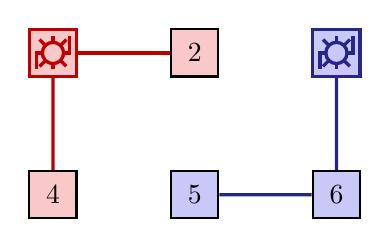
\begin{tikzpicture}[scale=0.6]

 % 設定
 \tikzset{customer/.style={rectangle,thick,draw=black,minimum height=0.6cm,minimum width=0.6cm}}
 \tikzset{on_switch/.style={rectangle,fill=black}}
 \tikzset{off_switch/.style={rectangle,draw=black,fill=white}}

 \definecolor{edge1}{RGB}{191,0,0}
 \definecolor{node1}{RGB}{249,200,200}
 \definecolor{edge3}{RGB}{38,38,134}
 \definecolor{node3}{RGB}{200,200,249}

 % 補助線
 % \draw [help lines,blue,step=1cm] (-5,0) grid (5,-5);
  
 % 需要家 customer
 \node[customer, draw=edge1, very thick, fill=node1] at (-3,0)(1){};
 \node[customer, fill=node1] at (0,0) (2){2};
 \node[customer, draw=edge3, very thick, fill=node3] at (3,0) (3){};
 \node[customer, fill=node1] at (-3,-3) (4){4};
 \node[customer, fill=node3] at (0,-3) (5){5};
 \node[customer, fill=node3] at (3,-3) (6){6};

 % substation1 (ホントはnewcommandでできるようにしたかった...)
 \draw [very thick, draw=edge1] (-3,0) circle [radius=0.225cm] node[minimum size=0.5cm](root1){};
 \draw [very thick, draw=edge1] (-2.775,0)--(-2.65,0)--(-2.65,0.35);
 \draw [very thick, draw=edge1] (-3.225,0)--(-3.35,0)--(-3.35,-0.35);
 \draw [very thick, draw=edge1] (-3,0.225)--(-3,0.35);
 \draw [very thick, draw=edge1] (-3,-0.225)--(-3,-0.35);
 \draw [very thick, draw=edge1] [domain=-0.284:-0.159] plot(\x-3,\x);
 \draw [very thick, draw=edge1] [domain=0.159:0.284] plot(\x-3,\x);
 \draw [very thick, draw=edge1] [domain=-0.284:-0.159] plot(\x-3,-\x);
 \draw [very thick, draw=edge1] [domain=0.159:0.284] plot(\x-3,-\x);

 % substation2
 \draw [very thick, draw=edge3] (3,0) circle [radius=0.225cm] node[minimum size=0.5cm](root2){};
 \draw [very thick, draw=edge3] (3.225,0)--(3.35,0)--(3.35,0.35);
 \draw [very thick, draw=edge3] (2.775,0)--(2.65,0)--(2.65,-0.35);
 \draw [very thick, draw=edge3] (3,0.225)--(3,0.35);
 \draw [very thick, draw=edge3] (3,-0.225)--(3,-0.35);
 \draw [very thick, draw=edge3] [domain=-0.284:-0.159] plot(\x+3,\x);
 \draw [very thick, draw=edge3] [domain=0.159:0.284] plot(\x+3,\x);
 \draw [very thick, draw=edge3] [domain=-0.284:-0.159] plot(\x+3,-\x);
 \draw [very thick, draw=edge3] [domain=0.159:0.284] plot(\x+3,-\x);

 % 辺
 % ルート
 %\draw [thick, draw=edge1] (root1) -- (1);
 %\draw [thick, draw=edge3] (root2) -- (3);
 % 繋がってない辺は点線
 \foreach \u / \v in {1/2, 1/4}
 \draw [very thick, draw=edge1] (\u) -- (\v);
 % 繋がってる辺は実線
 \foreach \u / \v in {3/6, 5/6}
 \draw [very thick, draw=edge3] (\u) -- (\v);


\end{tikzpicture}

%%%%%%%%%%%%%%%%%%%%%%%%%%%%%%%%%%%%%%%%%%%%%%%%%%%%%%%%%%
%%% Local Variables:
%%% mode: japanese-latex
%%% TeX-master: ``slide''
%%% End:
